\documentclass[]{article}
\usepackage{lmodern}
\usepackage{amssymb,amsmath}
\usepackage{ifxetex,ifluatex}
\usepackage{fixltx2e} % provides \textsubscript
\ifnum 0\ifxetex 1\fi\ifluatex 1\fi=0 % if pdftex
  \usepackage[T1]{fontenc}
  \usepackage[utf8]{inputenc}
\else % if luatex or xelatex
  \ifxetex
    \usepackage{mathspec}
  \else
    \usepackage{fontspec}
  \fi
  \defaultfontfeatures{Ligatures=TeX,Scale=MatchLowercase}
\fi
% use upquote if available, for straight quotes in verbatim environments
\IfFileExists{upquote.sty}{\usepackage{upquote}}{}
% use microtype if available
\IfFileExists{microtype.sty}{%
\usepackage{microtype}
\UseMicrotypeSet[protrusion]{basicmath} % disable protrusion for tt fonts
}{}
\usepackage[margin=1in]{geometry}
\usepackage{hyperref}
\hypersetup{unicode=true,
            pdftitle={Simulation of block decorrelation on chi-square data},
            pdfauthor={Xuelong Wang},
            pdfborder={0 0 0},
            breaklinks=true}
\urlstyle{same}  % don't use monospace font for urls
\usepackage{graphicx,grffile}
\makeatletter
\def\maxwidth{\ifdim\Gin@nat@width>\linewidth\linewidth\else\Gin@nat@width\fi}
\def\maxheight{\ifdim\Gin@nat@height>\textheight\textheight\else\Gin@nat@height\fi}
\makeatother
% Scale images if necessary, so that they will not overflow the page
% margins by default, and it is still possible to overwrite the defaults
% using explicit options in \includegraphics[width, height, ...]{}
\setkeys{Gin}{width=\maxwidth,height=\maxheight,keepaspectratio}
\IfFileExists{parskip.sty}{%
\usepackage{parskip}
}{% else
\setlength{\parindent}{0pt}
\setlength{\parskip}{6pt plus 2pt minus 1pt}
}
\setlength{\emergencystretch}{3em}  % prevent overfull lines
\providecommand{\tightlist}{%
  \setlength{\itemsep}{0pt}\setlength{\parskip}{0pt}}
\setcounter{secnumdepth}{5}
% Redefines (sub)paragraphs to behave more like sections
\ifx\paragraph\undefined\else
\let\oldparagraph\paragraph
\renewcommand{\paragraph}[1]{\oldparagraph{#1}\mbox{}}
\fi
\ifx\subparagraph\undefined\else
\let\oldsubparagraph\subparagraph
\renewcommand{\subparagraph}[1]{\oldsubparagraph{#1}\mbox{}}
\fi

%%% Use protect on footnotes to avoid problems with footnotes in titles
\let\rmarkdownfootnote\footnote%
\def\footnote{\protect\rmarkdownfootnote}

%%% Change title format to be more compact
\usepackage{titling}

% Create subtitle command for use in maketitle
\newcommand{\subtitle}[1]{
  \posttitle{
    \begin{center}\large#1\end{center}
    }
}

\setlength{\droptitle}{-2em}

  \title{Simulation of block decorrelation on chi-square data}
    \pretitle{\vspace{\droptitle}\centering\huge}
  \posttitle{\par}
    \author{Xuelong Wang}
    \preauthor{\centering\large\emph}
  \postauthor{\par}
      \predate{\centering\large\emph}
  \postdate{\par}
    \date{2018-09-21}

\usepackage{float,amsmath, bbm, siunitx, bm}
\floatplacement{figure}{H}
\newcommand{\indep}{\rotatebox[origin=c]{90}{$\models$}}

\begin{document}
\maketitle

{
\setcounter{tocdepth}{2}
\tableofcontents
}
\section{Motivation}\label{motivation}

We used resampling method to evaluate the proposed method performance.
However, there is an drawback of this resampling method That is the
decorrelation step is highly affected the sample size, especially when n
\textless{} p.~More specifically, when re-sampling size is too small,
the estimated inverse covariance matrix is way off the target. Thus,
that will affect the final result of the proposed method.

On possible solution is to modify the process of estimation of the
covariance matrix. For instance, we could only decorrelate part of the
covariate matrix i.e.~the main effect part or the interactive effect
part. we call it decorrelation by block. this process eventually will
reduce the number of parameters we are doing to estimate of the
covaraince matrix.

\section{Decorrelation by Block}\label{decorrelation-by-block}

Let \(X_t\) be the total covariate,

\[
  X_t = \begin{bmatrix}
          X_m \\
          X_i
        \end{bmatrix}
\]

Then the covariance matrix of \(X_t\) is

\[
  Var(X_t) = \begin{bmatrix}
              Var(X_m) & Cov(X_m, X_i) \\
              Cov(X_i, X_m) & Var(X_i) 
             \end{bmatrix}.
\]

Let A be the decorrelation matrix, we have

\[
  A = \begin{bmatrix}
       A_1 & 0 \\
       0 & A_2 
      \end{bmatrix},
\] where \(A_1 = \Sigma_{x_m}^{-1/2}\), and
\(A_2 = \Sigma_{x_i}^{-1/2}\)

To decorrelate a vector, we could left multiple \(A\) and \(X_t\),

\[
  AX_t = \begin{bmatrix}
           A_1 & 0 \\
           0 & A_2 
          \end{bmatrix} * \begin{bmatrix}
                            X_m \\
                            X_i
                          \end{bmatrix} = \begin{bmatrix}
                                            A_1X_m \\
                                            A_2X_i
                                          \end{bmatrix}.
\]

The covariance matrix of \(AX_t\) is

\[
  Var(X_t) = Var\left(\begin{bmatrix}
              A_1X_m \\
              A_2X_i
            \end{bmatrix}\right) = \begin{bmatrix}
                                     A_1\Sigma_{x_m}A_1^T & A_1Cov(X_m, X_i)A_2^T \\
                                     A_2Cov(X_i, X_m)A_1^2 & A_2\Sigma_{x_i}A_2^T 
                                    \end{bmatrix} = \begin{bmatrix}
                                                     I_m & A_1Cov(X_m, X_i)A_2^T \\
                                                     A_2Cov(X_i, X_m)A_1^2 & I_i
                                                    \end{bmatrix}.
\]

We could choose to only decorrelate the main effect or interactive
effect or both. The advantage is we don't care about the off diagonal
values, which will reduce the sensitivity of the process on the sample
size.

\section{Simulation result}\label{simulation-result}

\subsection{Chi-square with only main effects
decorrelated}\label{chi-square-with-only-main-effects-decorrelated}

\subsubsection{fixed main and fixed interactive
effect}\label{fixed-main-and-fixed-interactive-effect}

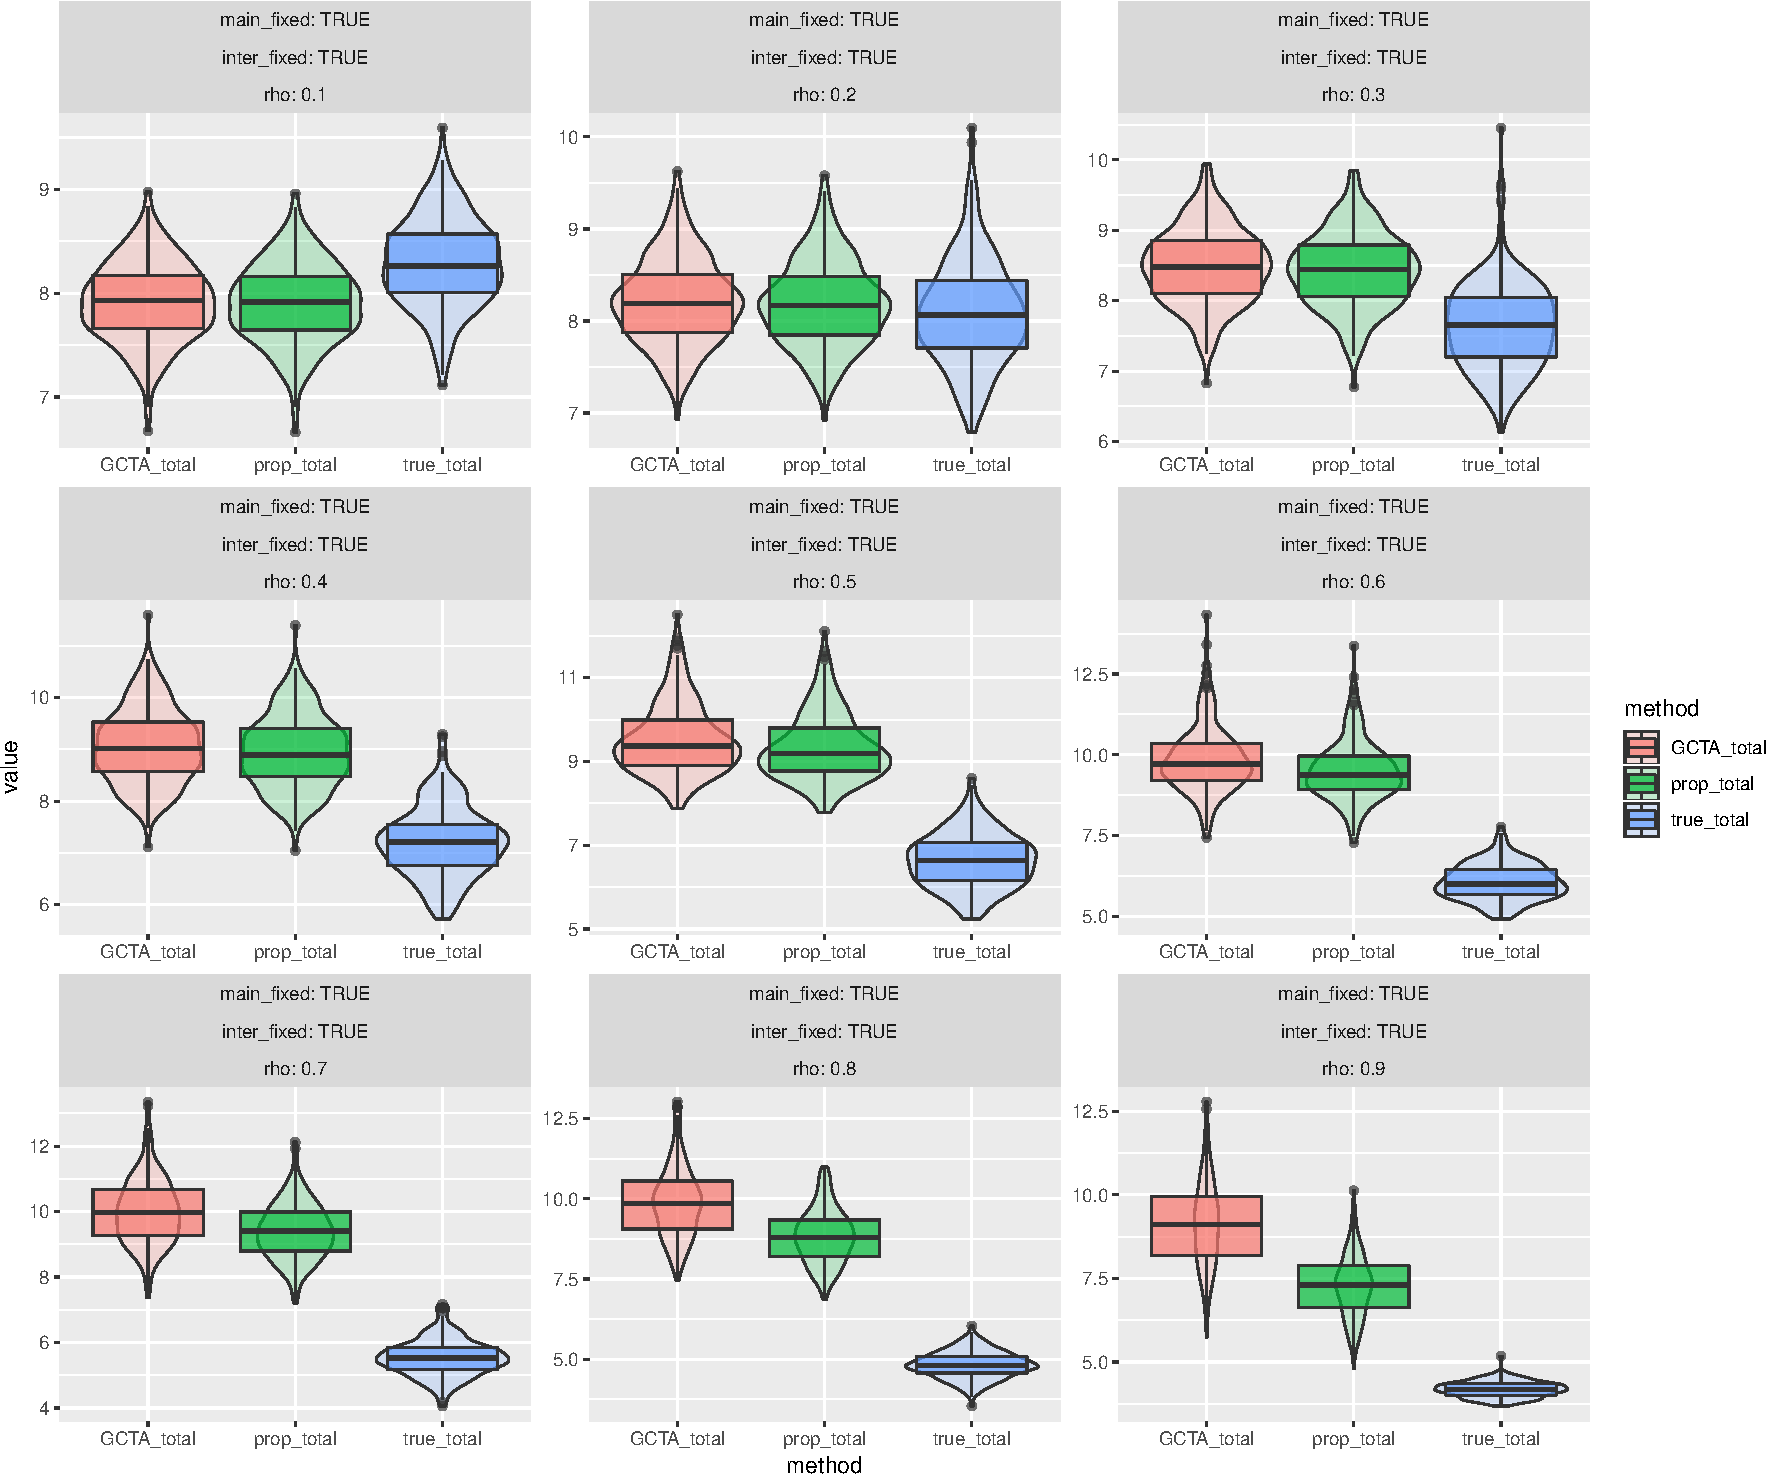
\includegraphics{block_decorrelation_report_files/figure-latex/fixed fixed only main-1.pdf}

\subsubsection{fixed main and random interactive
effect}\label{fixed-main-and-random-interactive-effect}

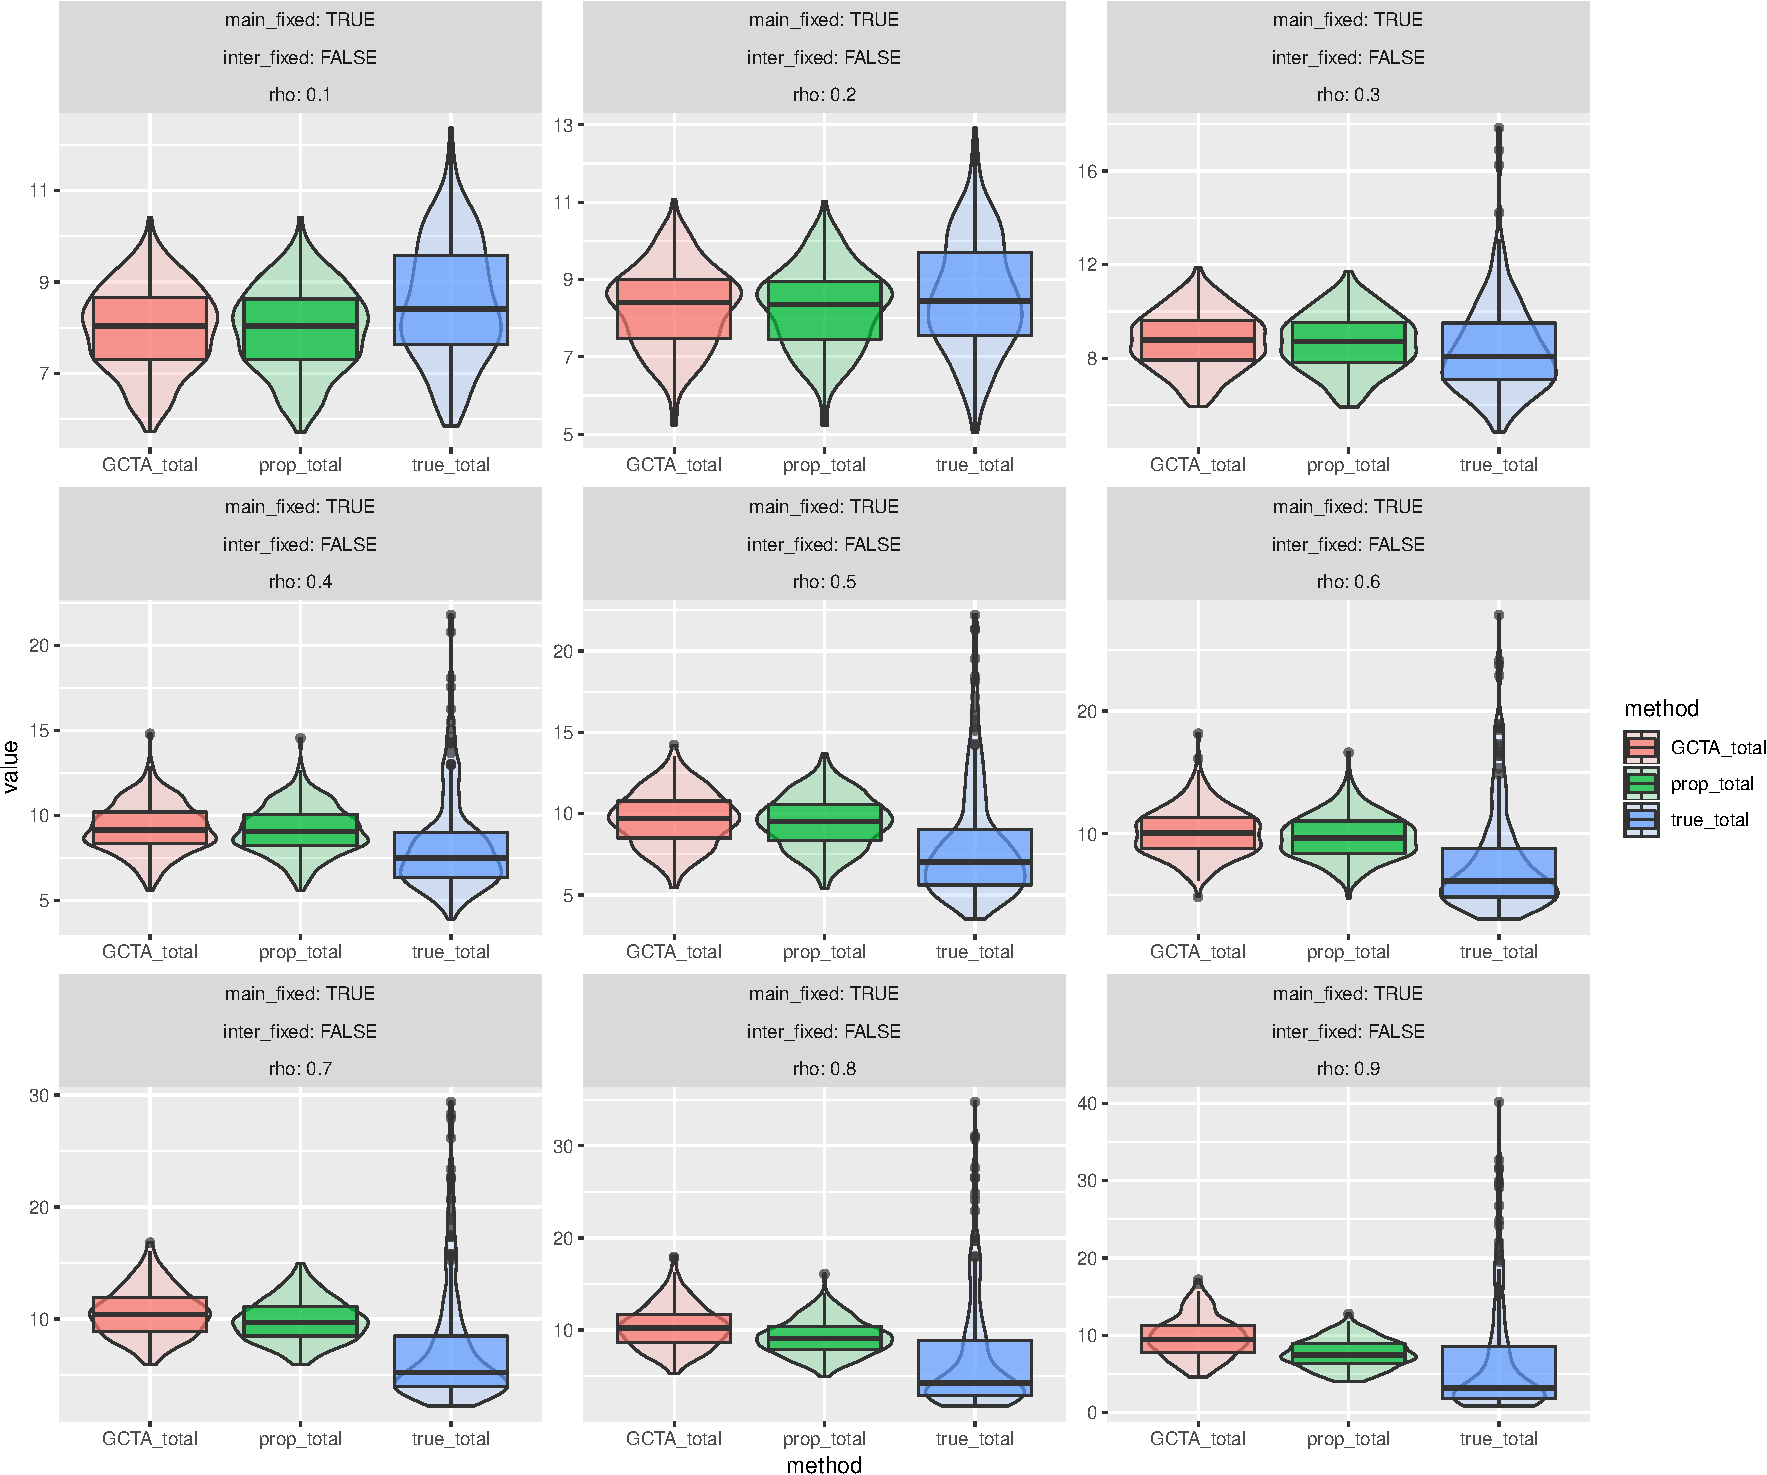
\includegraphics{block_decorrelation_report_files/figure-latex/fixed random only main-1.pdf}

\subsubsection{random main and random interactive
effect}\label{random-main-and-random-interactive-effect}

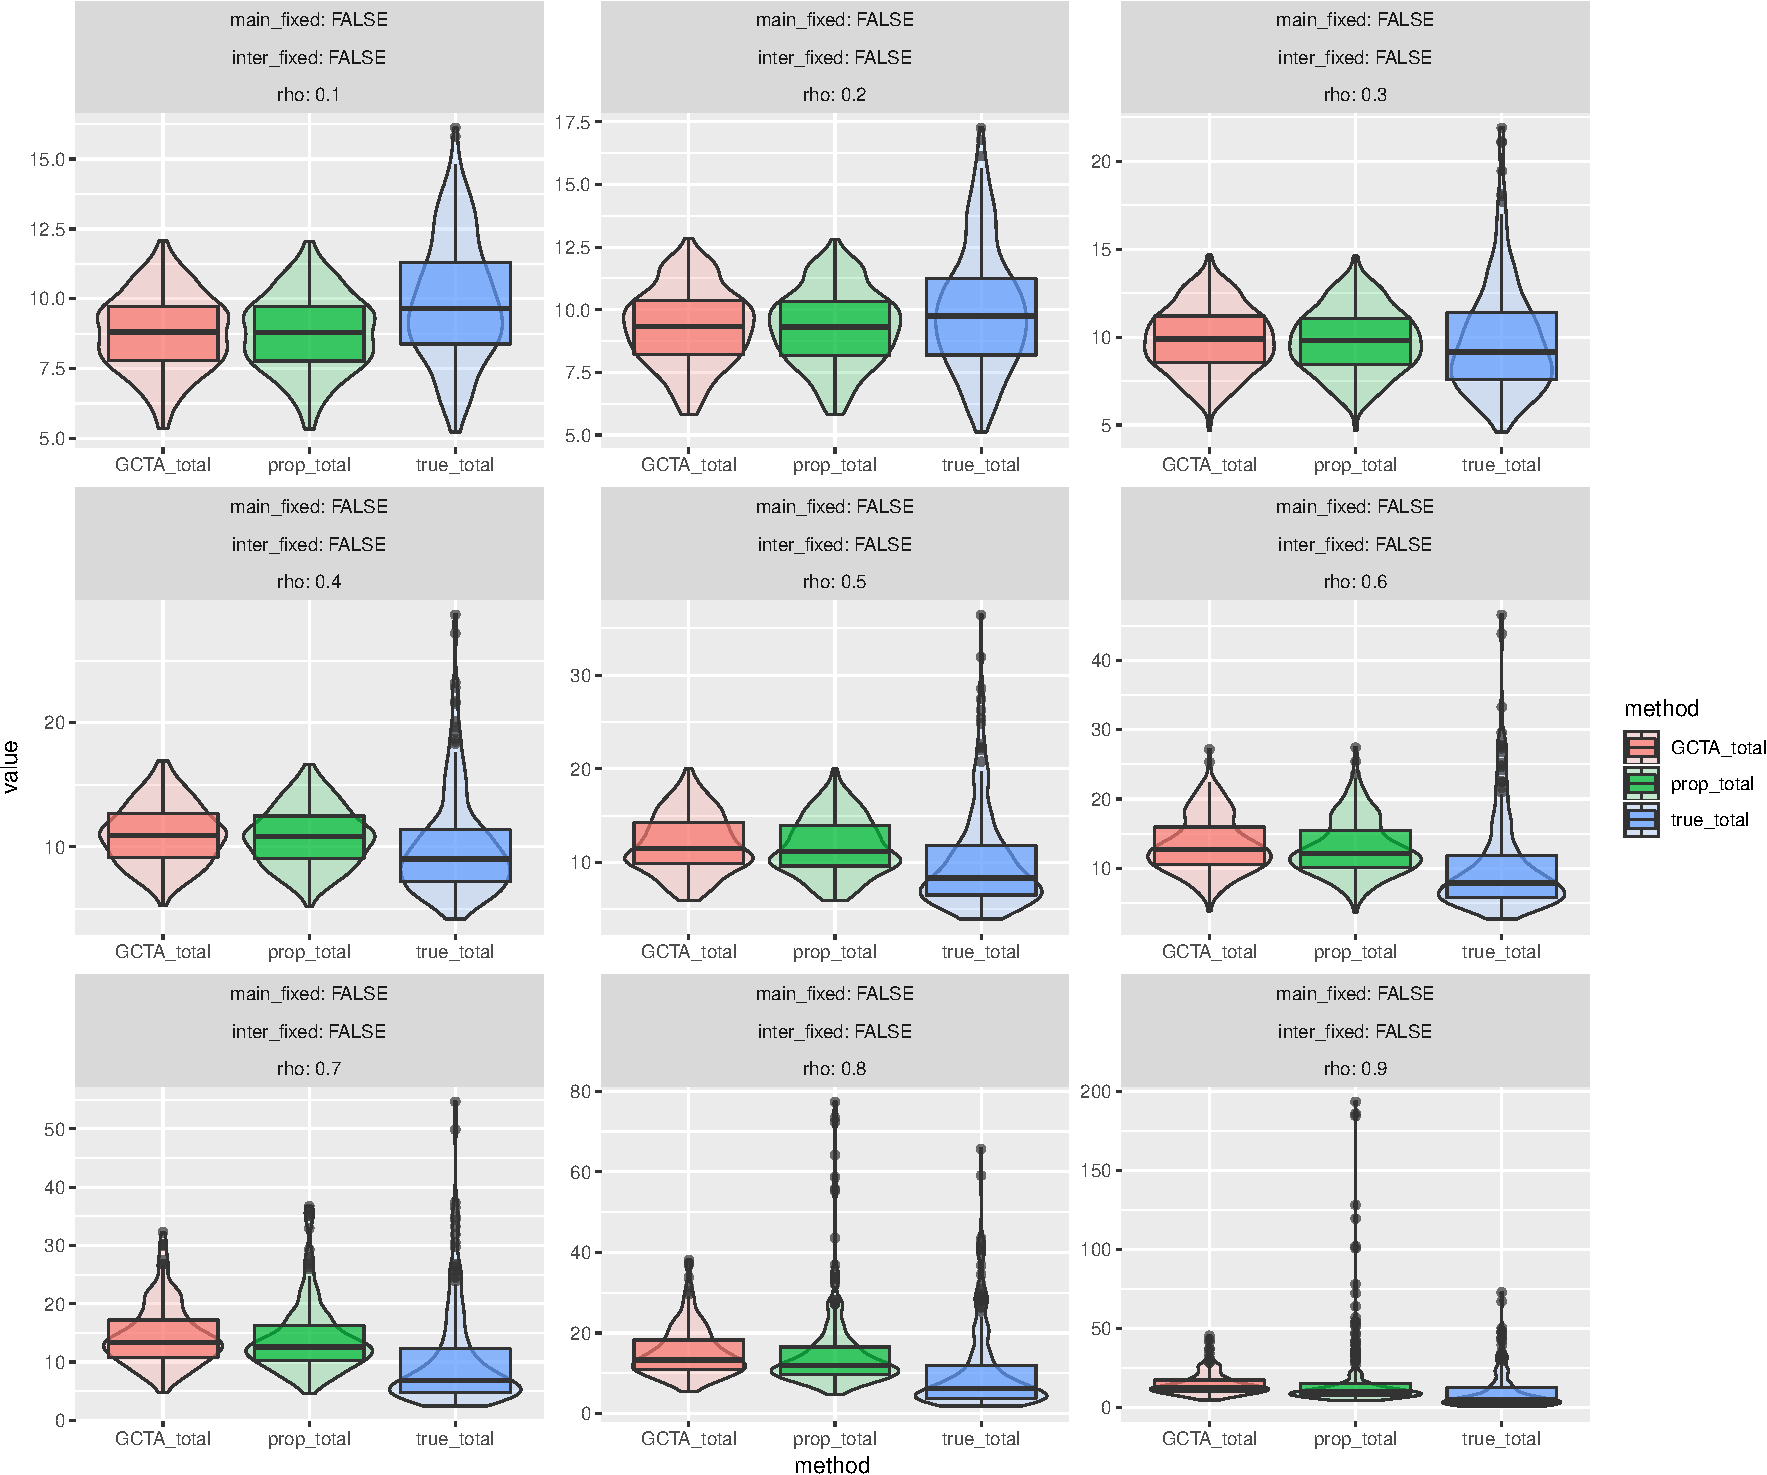
\includegraphics{block_decorrelation_report_files/figure-latex/random random only main-1.pdf}

\subsection{Chi-square with both main effects and inter effects
decorrelated}\label{chi-square-with-both-main-effects-and-inter-effects-decorrelated}

\subsubsection{fixed main and fixed interactive
effect}\label{fixed-main-and-fixed-interactive-effect-1}

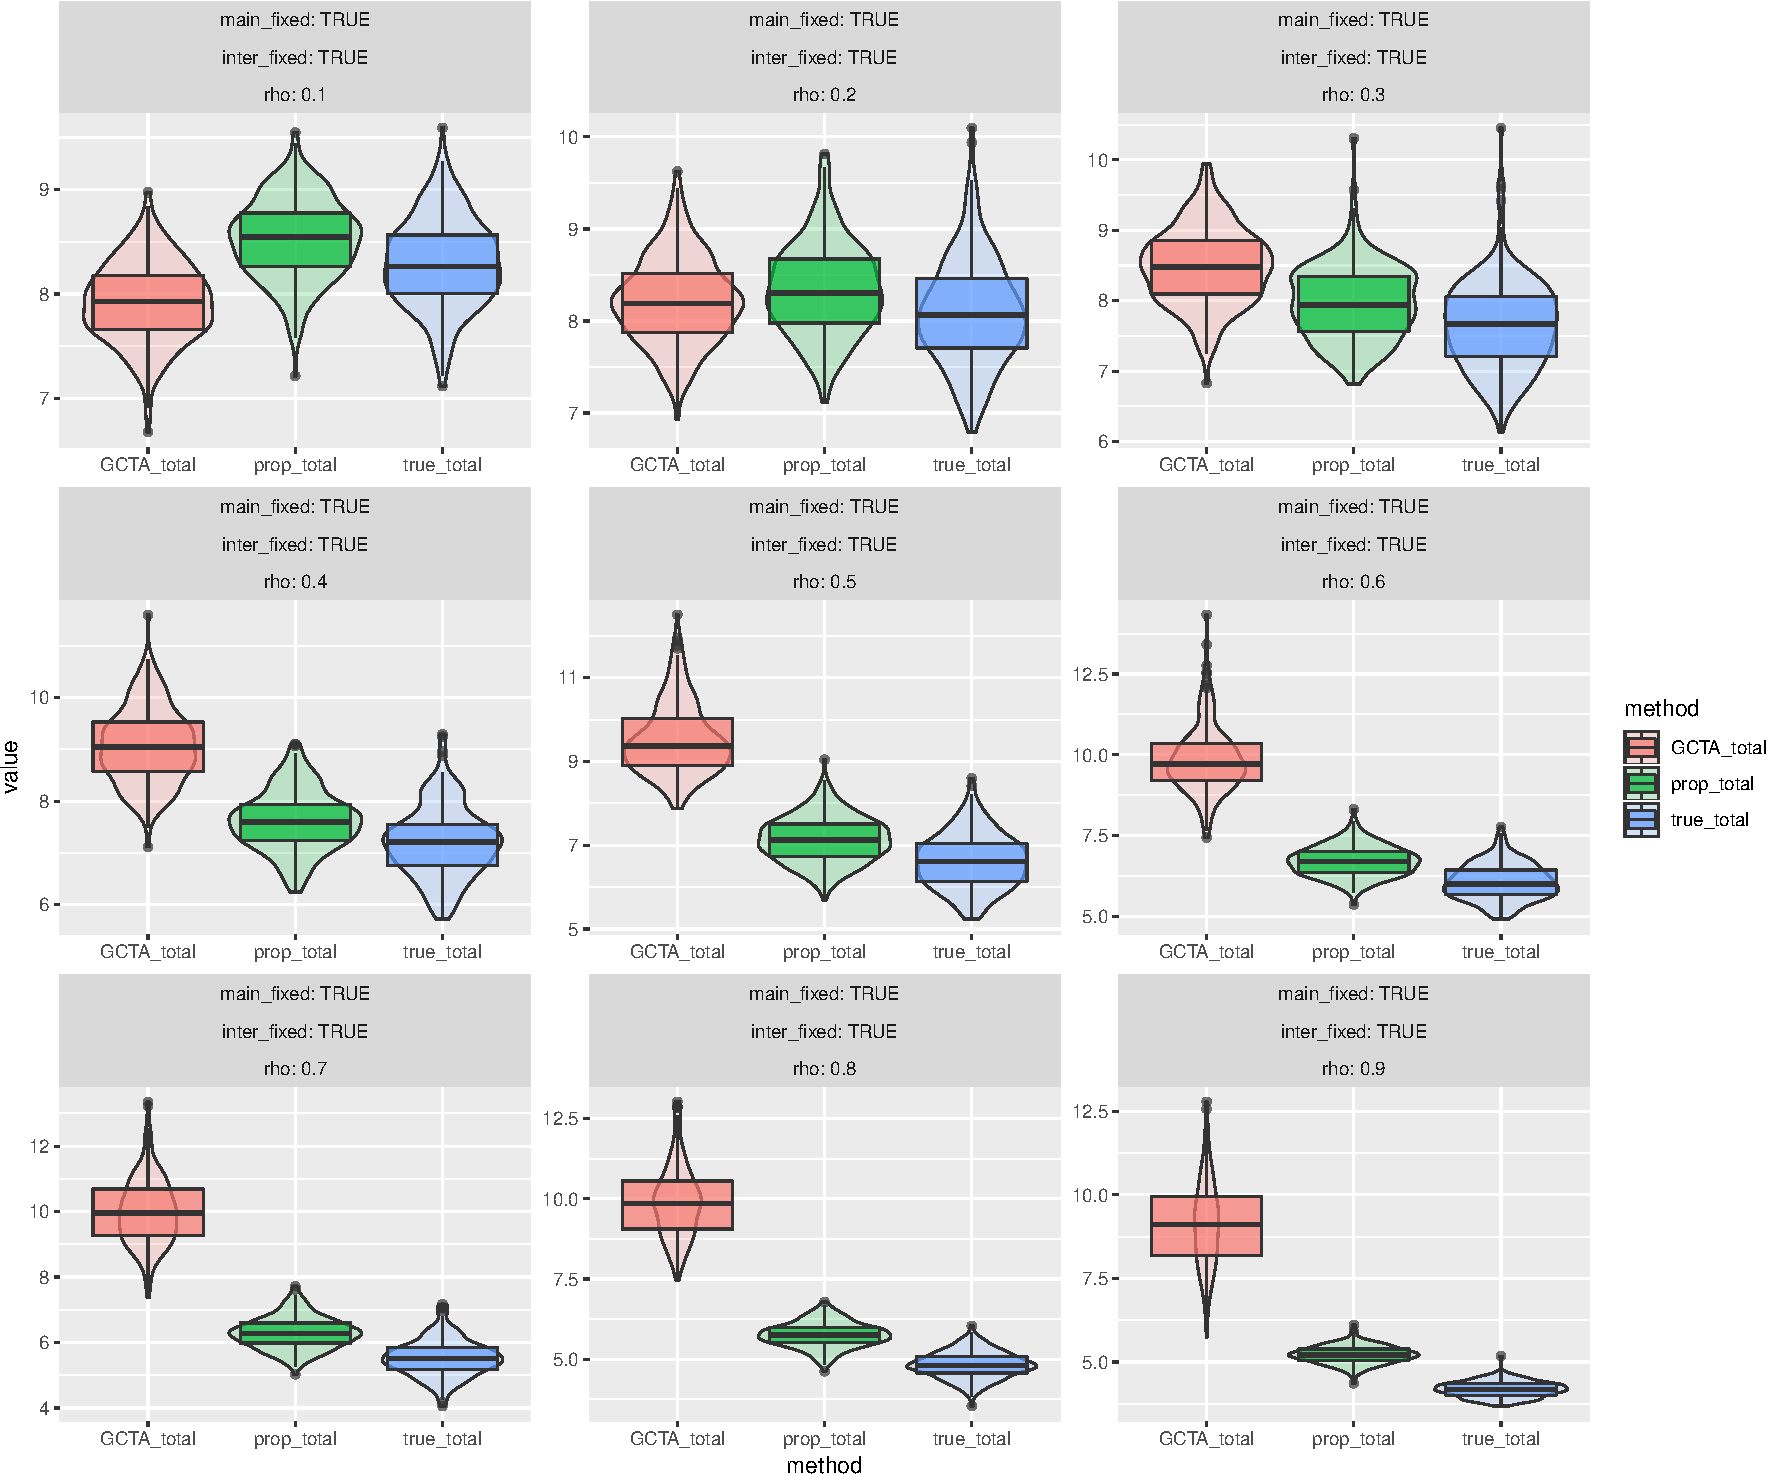
\includegraphics{block_decorrelation_report_files/figure-latex/fixed fixed both main and inter-1.pdf}


\end{document}
